\documentclass[conference]{IEEEtran}

\usepackage[T1]{fontenc}
\usepackage[utf8]{inputenc}
\usepackage{cite}
\usepackage{amsmath,amssymb,amsfonts}
\usepackage{graphicx}
\usepackage{booktabs}
\usepackage{multirow}
\usepackage{array}
\usepackage{siunitx}
\usepackage{url}
\usepackage{xcolor}
\usepackage{balance}

\title{Curriculum Reinforcement Learning for Variable-Height Balancing of a 10-Actuated Wheeled Biped Robot}

\author{
\IEEEauthorblockN{Van Thuong Nguyen}
\IEEEauthorblockA{
Your Institution\\
Email: vanthuong180702t@gmail.com
}
}

\begin{document}

\maketitle

\begin{abstract}
This paper presents a curriculum reinforcement learning framework for training a 10-actuated wheeled biped robot to balance at variable commanded torso heights. Each leg has five actuated joints: hip roll, hip yaw, hip pitch, knee, and wheel. The control policy is trained in MuJoCo MJX with JAX-accelerated vectorized simulation using proximal policy optimization (PPO). The policy receives a 40-dimensional observation that includes proprioceptive state and a normalized height command, and outputs joint-level targets that are converted to actuator torques through a PID low-level controller. To stabilize learning across a wide range of body heights, we employ a within-stage height curriculum that progressively expands the commanded height range from near the nominal standing posture toward deep crouching configurations based on a reward threshold criterion. A key component of the reward design is a height-consistent natural pose term that maps commanded height to target hip-pitch and knee angles via piecewise-linear interpolation, thereby preventing degenerate postures that satisfy height objectives through unnatural joint configurations. The framework also includes a multi-stage curriculum structure for future extension to stand-up recovery and robust push rejection, though the present work focuses on the variable-height balancing stage. We describe the full system design, reward formulation, curriculum strategy, and evaluation protocol, and present the framework as a foundation for further training and experimental validation.
\end{abstract}

\begin{IEEEkeywords}
Wheeled biped robot, reinforcement learning, curriculum learning, variable-height balancing, PID control, MuJoCo.
\end{IEEEkeywords}

\section{Introduction}
Wheeled biped robots combine the efficiency of wheel-based locomotion with the adaptability of legged morphology. Compared with conventional legged systems, wheeled bipeds can achieve lower-cost motion on flat terrain while exploiting articulated legs to modify body posture, regulate center-of-mass height, and improve disturbance rejection. However, these benefits come at the cost of more challenging control: balancing at different commanded heights requires managing the nonlinear coupling between wheel dynamics, torso attitude, and multi-joint leg motions.

Recent progress in reinforcement learning (RL) has shown that robust control policies can be learned directly in simulation for complex robotic systems~\cite{ppo}. Nevertheless, training a single policy to balance across a wide range of body heights is difficult due to poor sample efficiency and the risk of reward exploitation. In particular, simple height tracking rewards may allow policies to satisfy torso height objectives through unnatural or unstable joint configurations rather than through physically meaningful postures.

To address these challenges, we propose a curriculum reinforcement learning framework for a 10-actuated wheeled biped robot. The method explicitly conditions the policy on a target torso height and uses a within-stage height curriculum to progressively expand the difficulty from near-nominal standing to deep crouching. A height-consistent posture reward regularizes the joint configuration as a function of the commanded height, improving training stability and posture quality.

The main contributions of this work are:
\begin{itemize}
    \item A height-conditioned RL framework for variable-height balancing of a 10-actuated wheeled biped, with PID low-level control bridging policy outputs to actuator torques.
    \item A within-stage height curriculum that expands the commanded height range based on a reward threshold criterion, stabilizing learning across the full feasible height range.
    \item A height-consistent natural pose reward that ties hip-pitch and knee joint targets to the commanded torso height via piecewise-linear interpolation, preventing degenerate balancing strategies.
\end{itemize}

The framework additionally includes a multi-stage curriculum structure (stand-up recovery, robust push rejection) and an evaluation benchmark suite, though these extensions are not the focus of the present paper and remain as future work.

The rest of this paper is organized as follows. Section~II reviews related work. Section~III presents the robot platform and simulation setup. Section~IV formulates the learning problem. Section~V describes the reward design. Section~VI presents the curriculum strategy. Section~VII details the training pipeline and evaluation protocol. Section~VIII is reserved for experimental results. Section~IX discusses limitations and future work. Section~X concludes the paper.

\section{Related Work}
\label{sec:related}

Wheeled bipedal robots have been studied in several recent works. Klemm et al.~\cite{klemm2019ascento} developed Ascento, a two-wheeled jumping robot, demonstrating the feasibility of active balance control for wheeled bipeds. In subsequent work, Klemm et al.~\cite{klemm2020lqrwbc} proposed an LQR-assisted whole-body control approach for a wheeled bipedal robot with kinematic loops, achieving stable balancing through model-based control. Hsu et al.~\cite{hsu2022wbrfuzzy} applied fuzzy logic control to a wheeled biped for balance regulation. Li et al.~\cite{li2021wheelbiped} investigated dynamic wheeled motion control for wheel-biped transformable robots.

These approaches predominantly rely on model-based control or classical control techniques. In contrast, our work takes a learning-based approach using PPO~\cite{ppo} in a GPU-accelerated MuJoCo MJX~\cite{mujoco, mujoco_mjx_docs} simulation with JAX~\cite{jax}, which enables massively parallel training across thousands of environments. The key distinction of our framework is the combination of a height-conditioned policy, a progressive height curriculum, and a height-consistent posture reward that together address the challenge of stable balancing across a wide range of body heights.

\section{Robot Platform and Simulation Setup}

\subsection{Robot Morphology}
The robot considered in this work is a 10-actuated wheeled biped with five actuated joints on each leg: hip roll, hip yaw, hip pitch, knee, and wheel. The platform has a total mass of approximately \SI{8.1}{kg}, thigh length of \SI{0.26}{m}, shin length of \SI{0.28}{m}, wheel radius of \SI{0.06}{m}, and hip width of \SI{0.23}{m}. The sensing system includes one IMU and ten joint encoders. A physical robot with the same kinematic structure exists and is intended for future sim-to-real transfer, though hardware experiments are not part of the present work.

Let the joint vector be defined as
\begin{equation}
q_j =
\begin{bmatrix}
q_{\mathrm{hr}}^L &
q_{\mathrm{hy}}^L &
q_{\mathrm{hp}}^L &
q_{\mathrm{kn}}^L &
q_{\mathrm{wh}}^L &
q_{\mathrm{hr}}^R &
q_{\mathrm{hy}}^R &
q_{\mathrm{hp}}^R &
q_{\mathrm{kn}}^R &
q_{\mathrm{wh}}^R
\end{bmatrix}^\top,
\end{equation}
where the superscripts $L$ and $R$ denote the left and right legs, respectively.

\begin{figure}[t]
    \centering
    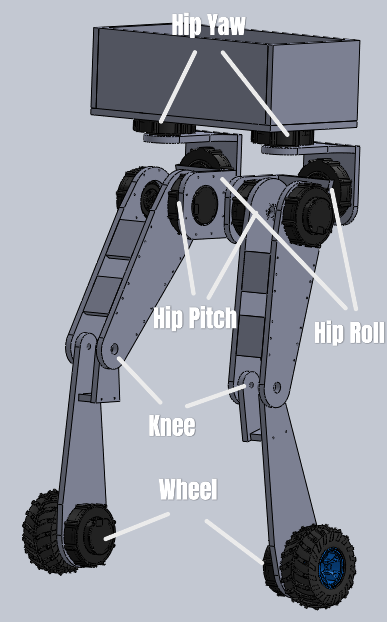
\includegraphics[width=0.72\linewidth]{figures/annotated_robot_joints.png}
    \caption{Mechanical structure and joint layout of the wheeled biped robot. Each leg has five actuated joints: hip roll, hip yaw, hip pitch, knee, and wheel. The left leg is annotated; the right leg is symmetric.}
    \label{fig:robot_joint_layout}
\end{figure}

Fig.~\ref{fig:robot_joint_layout} illustrates the mechanical structure and joint layout. The articulated hip and knee joints enable variable-height posture regulation, while the wheel joints provide balancing capability through active torque generation.

\subsection{Simulation Environment}
All policies are trained in MuJoCo MJX~\cite{mujoco, mujoco_mjx_docs} with JAX-based~\cite{jax} vectorized simulation. The physics simulation runs at \SI{500}{Hz} with timestep
\begin{equation}
\Delta t_{\mathrm{sim}} = \SI{0.002}{s},
\end{equation}
while the policy is queried at \SI{50}{Hz},
\begin{equation}
\Delta t_{\pi} = \SI{0.02}{s}.
\end{equation}
Each policy action is therefore held constant for ten simulation substeps. Training is parallelized across 4096 environments on GPU.

Domain randomization~\cite{tobin2017domain} is applied during training to improve robustness: body masses are perturbed by $\pm 10\%$, ground friction coefficients by $\pm 20\%$, and joint damping coefficients by $\pm 20\%$ relative to their nominal values.

\subsection{Low-Level PID Control}
\label{sec:pid}
Rather than mapping policy outputs directly to actuator torques, we employ a PID low-level controller that converts normalized policy targets into torque commands. This decouples the policy from raw torque generation and simplifies the learning problem.

The policy outputs $a_t \in [-1,1]^{10}$, which are interpreted differently depending on the joint type:
\begin{itemize}
    \item \textbf{Leg joints} (hip roll, hip yaw, hip pitch, knee): the policy output is linearly mapped to a position target within the joint range. A PD+I controller then computes the torque:
    \begin{equation}
    \tau_j = K_p^j (q_j^* - q_j) + K_d^j (0 - \dot{q}_j) + K_i^j \int (q_j^* - q_j)\, dt,
    \end{equation}
    where $q_j^*$ is the position target, $q_j$ and $\dot{q}_j$ are the measured joint position and velocity, and $K_p^j$, $K_d^j$, $K_i^j$ are per-joint gains. The integral term includes anti-windup clamping.
    \item \textbf{Wheel joints}: the policy output is mapped to a velocity target. A PI controller computes the torque:
    \begin{equation}
    \tau_w = K_p^w (\dot{q}_w^* - \dot{q}_w) + K_i^w \int (\dot{q}_w^* - \dot{q}_w)\, dt,
    \end{equation}
    where $\dot{q}_w^*$ is the velocity target and the derivative gain is zero ($K_d^w = 0$).
\end{itemize}

All torque outputs are clipped to the actuator limits. The PID gains are configured per joint and kept fixed during training. This controller is implemented as a reusable JAX-compatible module shared across all task environments.

\section{Problem Formulation}

\subsection{State, Observation, and Action}
At time step $t$, the robot state is $x_t = \{q_t, \dot{q}_t\}$, where $q_t$ and $\dot{q}_t$ are the generalized coordinates and velocities.

The policy receives a 40-dimensional observation vector
\begin{equation}
o_t = \big[g_t^b,\; v_t^b,\; \omega_t^b,\; q_{j,t},\; \dot{q}_{j,t},\; a_{t-1},\; \bar{h}_t^{cmd}\big] \in \mathbb{R}^{40},
\end{equation}
where:
\begin{itemize}
    \item $g_t^b \in \mathbb{R}^3$: gravity expressed in the body frame,
    \item $v_t^b \in \mathbb{R}^3$: body-frame linear velocity,
    \item $\omega_t^b \in \mathbb{R}^3$: body-frame angular velocity,
    \item $q_{j,t} \in \mathbb{R}^{10}$: joint positions,
    \item $\dot{q}_{j,t} \in \mathbb{R}^{10}$: joint velocities,
    \item $a_{t-1} \in \mathbb{R}^{10}$: previous policy action,
    \item $\bar{h}_t^{cmd} \in \mathbb{R}$: normalized height command.
\end{itemize}

The normalized height command is defined as
\begin{equation}
\bar{h}_t^{cmd} = \frac{h_t^{cmd} - h_{\min}}{h_{\max} - h_{\min}},
\label{eq:height_norm}
\end{equation}
where $h_{\min} = \SI{0.40}{m}$ and $h_{\max} = \SI{0.70}{m}$ for the balance task. These bounds correspond to the kinematically feasible standing height range of the robot.

Observations are normalized online using Welford's running mean and variance estimator~\cite{welford1962}, which is updated during training but held fixed during evaluation.

The policy outputs a normalized action $a_t = \pi_\theta(o_t) \in [-1,1]^{10}$, which is converted to actuator torques through the PID controller described in Section~\ref{sec:pid}.

\subsection{Learning Objective}
We seek a policy $\pi_\theta$ that maximizes the expected discounted return
\begin{equation}
J(\theta)=\mathbb{E}_{\pi_\theta}\left[\sum_{t=0}^{T-1}\gamma^t r_t\right],
\end{equation}
where $\gamma = 0.99$ is the discount factor and $r_t$ is the reward at step $t$.

Training is performed using PPO~\cite{ppo} with clipped surrogate objective
\begin{equation}
L^{\mathrm{PPO}}(\theta) =
\mathbb{E}_t\left[
\min\left(
\rho_t(\theta)\hat{A}_t,\;
\mathrm{clip}\big(\rho_t(\theta), 1-\epsilon, 1+\epsilon\big)\hat{A}_t
\right)
\right],
\end{equation}
where $\rho_t(\theta)=\pi_\theta(a_t|o_t)/\pi_{\theta_{\mathrm{old}}}(a_t|o_t)$ and $\epsilon=0.2$. The full objective includes a clipped value loss (coefficient 0.5) and entropy regularization (coefficient 0.01). Advantages $\hat{A}_t$ are computed using Generalized Advantage Estimation (GAE)~\cite{gae} with $\lambda=0.95$.

\section{Reward Design}
\label{sec:reward}

\subsection{Reward Structure}
The total reward at each step is a weighted sum of positive reward terms and penalty terms:
\begin{equation}
r_t = \sum_i w_i r_t^{(i)},
\label{eq:reward_total}
\end{equation}
where $w_i$ is the weight for component $r_t^{(i)}$. Some components are positive rewards (encouraging desired behavior) and others are penalties (discouraging undesired behavior, with negative weights). The complete set of reward terms and their weights for the balance task are given in Table~\ref{tab:reward_weights}.

\begin{table}[t]
\centering
\caption{Reward components and weights for the variable-height balance task.}
\label{tab:reward_weights}
\begin{tabular}{l l r}
\toprule
Component & Type & Weight \\
\midrule
Height tracking ($r_{\mathrm{height}}$) & Positive & 2.5 \\
Body level ($r_{\mathrm{level}}$) & Positive & 1.5 \\
Position drift ($r_{\mathrm{drift}}$) & Positive & 1.5 \\
Heading ($r_{\mathrm{heading}}$) & Positive & 0.5 \\
Leg symmetry ($r_{\mathrm{sym}}$) & Positive & 0.5 \\
Legs forward ($r_{\mathrm{fwd}}$) & Positive & 0.5 \\
Legs vertical ($r_{\mathrm{vert}}$) & Positive & 0.5 \\
No motion ($r_{\mathrm{still}}$) & Positive & 0.5 \\
Angular stability ($r_{\mathrm{orient}}$) & Positive & 0.5 \\
Yaw suppression ($r_{\mathrm{yaw}}$) & Positive & 0.5 \\
Natural pose ($r_{\mathrm{nat}}$) & Positive & 0.4 \\
Alive bonus ($r_{\mathrm{alive}}$) & Positive & 0.3 \\
Action rate ($p_{\Delta a}$) & Penalty & $-0.03$ \\
Wheel velocity ($p_{\mathrm{wh}}$) & Penalty & $-0.0008$ \\
Joint torque ($p_\tau$) & Penalty & $-0.0005$ \\
Joint velocity ($p_{\dot{q}}$) & Penalty & $-0.0006$ \\
\bottomrule
\end{tabular}
\end{table}

\subsection{Primary Reward Terms}

\subsubsection{Body-Level Reward}
To encourage the torso to remain parallel to the ground, we define
\begin{equation}
r_{\mathrm{level}} =
\exp\left(-\frac{\phi_t^2}{\sigma_r^2}\right)
\exp\left(-\frac{\theta_t^2}{\sigma_p^2}\right),
\label{eq:body_level}
\end{equation}
where $\phi_t$ and $\theta_t$ are the torso roll and pitch angles, and $\sigma_r = \sigma_p = 0.15\,\mathrm{rad}$.

\subsubsection{Height Tracking Reward}
The torso height is encouraged to match the commanded height:
\begin{equation}
r_{\mathrm{height}} =
\exp\left(
-\frac{(h_t - h_t^{cmd})^2}{\sigma_h^2}
\right),
\label{eq:height_reward}
\end{equation}
with $\sigma_h = 0.25\,\mathrm{m}$, providing a gradient signal even when the actual height is far from the target.

\subsubsection{Heading and Position Regularization}
To keep the robot near its initial yaw $\psi_0$ and anchor position $p_{xy,0}$:
\begin{equation}
r_{\mathrm{heading}} =
\exp\left(
-\frac{\mathrm{wrap}(\psi_t - \psi_0)^2}{\sigma_\psi^2}
\right),
\label{eq:heading_reward}
\end{equation}
\begin{equation}
r_{\mathrm{drift}} =
\exp\left(
-\frac{\|p_{xy,t} - p_{xy,0}\|_2^2}{\sigma_d^2}
\right),
\label{eq:drift_reward}
\end{equation}
with $\sigma_\psi = 0.5\,\mathrm{rad}$ and $\sigma_d = 1.0\,\mathrm{m}$.

\subsubsection{Angular Stability}
To reduce torso oscillation:
\begin{equation}
r_{\mathrm{orient}} =
\mathrm{clip}\left(1 - 0.15 \|\omega_t^b\|_2,\; 0,\; 1\right),
\label{eq:orient_reward}
\end{equation}
and a dedicated yaw suppression term:
\begin{equation}
r_{\mathrm{yaw}} =
\mathrm{clip}\left(1 - 0.5 |\omega_{z,t}^b|,\; 0,\; 1\right).
\label{eq:yaw_reward}
\end{equation}

\subsubsection{Leg Symmetry}
To encourage symmetric leg postures:
\begin{equation}
r_{\mathrm{sym}} =
\exp\left(
-\frac{
\left\|
q_{\mathrm{leg},t}^L - q_{\mathrm{leg},t}^R
\right\|_2^2
}{\sigma_{sym}^2}
\right),
\label{eq:symmetry_reward}
\end{equation}
where $q_{\mathrm{leg}}^{L/R}$ includes hip roll, hip yaw, hip pitch, and knee for each leg, and $\sigma_{sym} = 0.5$.

\subsubsection{No-Motion Reward}
To encourage the robot to remain stationary:
\begin{equation}
r_{\mathrm{still}} =
\exp\left(
-\frac{\|v_t^b\|_2^2}{\sigma_v^2}
\right),
\label{eq:no_motion}
\end{equation}
with $\sigma_v = 0.2\,\mathrm{m/s}$. This term is assigned a high weight during pure balance training (weight 0.5) but would be reduced or removed for locomotion or push-recovery tasks where motion is necessary.

\subsection{Height-Consistent Natural Pose Reward}
\label{sec:natural_pose}
A key design of our method is a posture regularization term that enforces consistency between the commanded torso height and the desired leg configuration. Let the desired hip-pitch and knee angles be $q_{\mathrm{hp}}^*(h^{cmd})$ and $q_{\mathrm{kn}}^*(h^{cmd})$, computed using piecewise-linear interpolation.

The interpolation is defined over the extended kinematic range $h^{cmd} \in [0.38, 0.72]\,\mathrm{m}$, divided at the nominal standing keyframe $h = 0.71\,\mathrm{m}$. During BalanceEnv training the commanded height is sampled in $[0.40, 0.70]\,\mathrm{m}$, so the function operates entirely within the lower segment; the upper segment $[0.71, 0.72]\,\mathrm{m}$ is defined for generality.

For high standing heights $h^{cmd}\in[0.71,0.72]\,\mathrm{m}$:
\begin{equation}
t_h = \frac{h^{cmd} - 0.71}{0.72 - 0.71},
\end{equation}
\begin{equation}
q_{\mathrm{hp}}^* = 0.3 + t_h(0.0 - 0.3),
\qquad
q_{\mathrm{kn}}^* = 0.5 + t_h(0.0 - 0.5).
\end{equation}

For lower heights $h^{cmd}\in[0.38,0.71]\,\mathrm{m}$:
\begin{equation}
t_l = \frac{h^{cmd} - 0.38}{0.71 - 0.38},
\end{equation}
\begin{equation}
q_{\mathrm{hp}}^* = 1.5 + t_l(0.3 - 1.5),
\qquad
q_{\mathrm{kn}}^* = 2.5 + t_l(0.5 - 2.5).
\end{equation}

The posture error is
\begin{equation}
e_{\mathrm{pose}} =
\Big(
(q_{\mathrm{hp}}^L - q_{\mathrm{hp}}^*)^2
+
(q_{\mathrm{hp}}^R - q_{\mathrm{hp}}^*)^2
+
(q_{\mathrm{kn}}^L - q_{\mathrm{kn}}^*)^2
+
(q_{\mathrm{kn}}^R - q_{\mathrm{kn}}^*)^2
\Big)^{1/2}.
\end{equation}
The natural pose reward is
\begin{equation}
r_{\mathrm{nat}} =
\exp\left(
-\frac{e_{\mathrm{pose}}^2}{\sigma_{nat}^2}
\right)
r_{\mathrm{knee}},
\label{eq:natural_pose}
\end{equation}
where $\sigma_{nat} = 0.8$ and $r_{\mathrm{knee}}$ penalizes knee hyperextension:
\begin{equation}
r_{\mathrm{knee}}=
\exp\left(-\frac{\min(q_{\mathrm{kn}}^L,0)^2}{\sigma_k^2}\right)
\exp\left(-\frac{\min(q_{\mathrm{kn}}^R,0)^2}{\sigma_k^2}\right).
\end{equation}

This reward is important because it prevents the robot from exploiting unnatural crouching or unstable joint postures merely to satisfy torso height objectives. Without it, the policy could learn to achieve a target height through, for example, extreme hip abduction with nearly straight legs rather than through a kinematically natural bent-knee configuration.

\subsection{Effort and Smoothness Penalties}
We regularize torque magnitude, joint velocity, action variation, and wheel rotation:
\begin{equation}
p_\tau = \sum_{j=1}^{10} \tau_{t,j}^2, \quad
p_{\dot{q}} = \sum_{j=1}^{10} \dot{q}_{j,t}^2, \quad
p_{\Delta a} = \sum_{j=1}^{10}(a_{t,j} - a_{t-1,j})^2,
\end{equation}
\begin{equation}
p_{\mathrm{wh}} = \dot{q}_{\mathrm{wh},t}^{L\,2} + \dot{q}_{\mathrm{wh},t}^{R\,2}.
\end{equation}
The wheel velocity penalty encourages the robot to balance without relying on continuous wheel spinning, which is desirable for stationary balance.

\subsection{Termination Conditions}
An episode terminates early if the torso tilt exceeds $0.8\,\mathrm{rad}$ ($\approx 46^\circ$) or the torso height drops below $0.3\,\mathrm{m}$. Otherwise, episodes run for 1000 steps (20 seconds of simulated time). A survival bonus $r_{\mathrm{alive}} \in \{0, 1\}$ is given at each non-terminal step (weight 0.3 in the balance task), providing a constant per-step incentive to remain standing.

\section{Curriculum Learning Strategy}
\label{sec:curriculum}

\subsection{Within-Stage Height Curriculum}
Rather than sampling the commanded height from the full feasible range from the beginning, we employ a within-stage curriculum~\cite{bengio2009curriculum} that progressively expands the lower bound of the height command distribution.

The height lower bound is decreased by a fixed step $\delta_h$ whenever performance exceeds a threshold $r_{\mathrm{thr}}$:
\begin{equation}
h_{\min}^{(k+1)} = \max\!\big(h_{\min}^{(k)} - \delta_h,\; h_{\min}^{final}\big),
\quad \text{if } \bar{r}_{\mathrm{eval}} \geq r_{\mathrm{thr}}.
\label{eq:height_curriculum}
\end{equation}

The advancement signal $\bar{r}_{\mathrm{eval}}$ is obtained from a dedicated evaluation pass: every $I_{\mathrm{eval}} = 50$ training updates, the current policy is evaluated greedily (no exploration noise) over 20 complete episodes using 32 parallel environments, with the observation normalizer held fixed. The per-step return is then
\begin{equation}
\bar{r}_{\mathrm{eval}} = \frac{R_{\mathrm{mean}}}{T},
\label{eq:eval_per_step}
\end{equation}
where $R_{\mathrm{mean}}$ is the mean episode return and $T = 1000$ is the episode length. Advancement fires when $\bar{r}_{\mathrm{eval}} \geq r_{\mathrm{thr}}$. Using a greedy evaluation pass rather than the noisy per-update training reward produces a more reliable signal for curriculum advancement decisions.

In our implementation, the initial lower bound is $h_{\min}^{init} = \SI{0.69}{m}$ (close to the nominal standing keyframe), the final lower bound is $h_{\min}^{final} = \SI{0.40}{m}$, the curriculum has $N_c = 29$ discrete levels with step size $\delta_h = (h_{\min}^{init} - h_{\min}^{final})/N_c \approx \SI{0.01}{m}$, and the threshold is set at $r_{\mathrm{thr}} = 0.85$. At each level, the height command is sampled uniformly:
\begin{equation}
h_t^{cmd}\sim \mathcal{U}\big(h_{\min}^{(k)},\; h_{\max}\big),
\end{equation}
where $h_{\max} = \SI{0.70}{m}$.

This curriculum stabilizes early learning by first focusing on heights near the nominal standing posture before progressively expanding toward deep crouching configurations that require larger joint excursions.

\subsection{Multi-Stage Curriculum (Future Work)}
\label{sec:multi_stage}
The codebase includes a multi-stage curriculum manager that can chain training stages with warm-starting and performance-gated promotion/demotion. The planned stages are:
\begin{enumerate}
    \item \textbf{Stage 1: Variable-height balancing} (the focus of this paper).
    \item \textbf{Stage 2: Stand-up recovery and height transitions.} The robot would learn to transition between heights and recover from fallen initial states using a mixed initialization scheme.
    \item \textbf{Stage 3: Robust balancing under external pushes.} The balance policy would be fine-tuned with periodic random push forces ($F_{push} = \SI{40}{N}$) applied to the torso.
\end{enumerate}

Stage promotion is gated by a held-out evaluation metric (mean episode return from a greedy evaluation pass), not by noisy training-time rewards. Stages 2 and 3 have corresponding environment implementations and training configurations but have not yet been trained or evaluated. Their results are therefore not reported in this paper.

\section{Training Pipeline and Evaluation Protocol}

\subsection{Network Architecture}
The policy and value function share the same architecture: separate multi-layer perceptrons (MLPs) with hidden layer sizes $\{256, 256, 128\}$ and ELU activation, implemented using Flax~\cite{flax}. Weights are initialized using orthogonal initialization. The policy network outputs the mean of a Gaussian distribution over actions, with a learned log-standard-deviation parameter initialized to $\log(0.2)$.

\subsection{Training Configuration}
Training uses PPO with 4096 parallel environments, a rollout length of 128 steps, 4 epochs per update, 32 minibatches, learning rate $2 \times 10^{-4}$ with Adam optimizer, and gradient clipping at global norm 0.5. Each training run targets approximately $10^7$ environment steps. Observation normalization uses a Welford running mean/variance estimator that is updated during training rollouts and frozen during evaluation.

\subsection{Evaluation Protocol}
The evaluation framework provides four benchmark modes:
\begin{enumerate}
    \item \textbf{Nominal:} Standard balance evaluation without perturbation.
    \item \textbf{Push recovery:} Balance under periodic random push forces.
    \item \textbf{Domain randomized:} Balance with perturbed mass and friction.
    \item \textbf{Command tracking:} Sweep over commanded heights and report per-height tracking error.
\end{enumerate}

For each mode, the following metrics are reported:
\begin{itemize}
    \item Mean and standard deviation of episode return,
    \item Task success rate (fraction of episodes surviving the full duration),
    \item Fall rate (fraction of episodes terminated by tilt or height violation).
\end{itemize}

For the command tracking mode, the height tracking error is
\begin{equation}
e_h = \frac{1}{T}\sum_{t=1}^{T} |h_t - h_t^{cmd}|,
\end{equation}
and the average torso tilt is
\begin{equation}
e_{\mathrm{tilt}} =
\frac{1}{T}\sum_{t=1}^{T}\sqrt{\phi_t^2+\theta_t^2}.
\end{equation}

In addition to reward-based metrics, a standing quality analysis module checks for reward exploitation patterns by monitoring: excessive wheel spin, height oscillation, position drift, chronic lean, control jitter, leg asymmetry, and torso wobble. These quality signals help detect degenerate policies that achieve high reward through unintended strategies.

\section{Experimental Results}
\label{sec:results}

\textit{Note: Training has not yet been completed. This section will be filled with quantitative results after the balance policy is trained and evaluated. The placeholders below indicate the planned experiments and metrics.}

\subsection{Learning Curves}
[TODO: Add learning curve figure showing reward vs.\ training steps, including curriculum level progression over time.]

\subsection{Variable-Height Balancing Results}
\begin{table}[ht]
\centering
\caption{Variable-height balancing performance at different commanded heights.}
\label{tab:balance_results}
\begin{tabular}{c c c c}
\toprule
Height (m) & Height Error (m) & Tilt Error (rad) & Success Rate (\%) \\
\midrule
0.40 & [TODO] & [TODO] & [TODO] \\
0.45 & [TODO] & [TODO] & [TODO] \\
0.55 & [TODO] & [TODO] & [TODO] \\
0.65 & [TODO] & [TODO] & [TODO] \\
0.70 & [TODO] & [TODO] & [TODO] \\
\bottomrule
\end{tabular}
\end{table}

[TODO: Add figure showing robot snapshots at multiple commanded heights.]

\subsection{Ablation: Natural Pose Reward}
[TODO: Train two policies---one with and one without the natural pose reward ($r_{\mathrm{nat}}$)---and compare height tracking error, posture quality, and convergence speed. This ablation is critical for validating the main methodological contribution.]

\subsection{Effort and Smoothness}
[TODO: Report RMS torque and action smoothness metrics:
\begin{equation}
\mathrm{RMS}_{\tau}=
\sqrt{
\frac{1}{10T}
\sum_{t=1}^{T}
\sum_{j=1}^{10}
\tau_{t,j}^2
},
\qquad
S_{a}=
\frac{1}{10T}
\sum_{t=1}^{T}
\sum_{j=1}^{10}
(a_{t,j}-a_{t-1,j})^2.
\end{equation}
]

\section{Discussion and Limitations}
\label{sec:discussion}

\subsection{Framework Design}
The main design principle of the proposed framework is to decompose the variable-height balancing problem into a progressive curriculum that stabilizes learning by starting near the nominal standing pose and expanding toward more challenging configurations. The height-consistent natural pose reward complements this by constraining the joint-space solution to physically meaningful postures at each target height, which we hypothesize reduces reward exploitation and improves training stability.

The PID low-level controller serves as an important interface between the RL policy and the physics simulation. By having the policy output position/velocity targets rather than raw torques, the effective action space is better conditioned and the policy can focus on high-level posture regulation rather than low-level torque generation.

\subsection{Current Limitations}
This work has several important limitations that should be noted:

\begin{enumerate}
    \item \textbf{No trained results yet.} The framework has been fully implemented and tested at the unit and integration level, but complete training runs have not been executed at the time of writing. All experimental results sections contain placeholders. The claims in this paper are therefore about the framework design, not about demonstrated performance.

    \item \textbf{Balance only.} The present work focuses exclusively on stationary variable-height balancing. Stand-up recovery (Stage~2) and robust push rejection (Stage~3) have corresponding code and configurations but have not been trained. Dynamic locomotion is not addressed.

    \item \textbf{No sim-to-real transfer.} All work is conducted in simulation. Although the robot model matches a physical platform, sim-to-real transfer has not been attempted.

    \item \textbf{No baseline comparisons.} The current results do not include comparisons against classical control methods (e.g., LQR) or alternative RL formulations (e.g., without curriculum, without PID, without natural pose reward). Ablation studies are planned but not yet conducted.

    \item \textbf{Single seed.} Planned training runs do not yet include multi-seed experiments, which are needed for statistical validity.

    \item \textbf{Height curriculum evaluation is lightweight.} The within-stage height curriculum now uses a greedy evaluation pass (32 envs × 20 episodes every 50 updates) rather than noisy training-rollout rewards, reducing the risk of premature advancement. However, the evaluation budget is small, and the signal may still be noisy in early training before the policy stabilizes.
\end{enumerate}

\section{Conclusion}
This paper presented a curriculum reinforcement learning framework for variable-height balancing of a 10-actuated wheeled biped robot. The framework includes a height-conditioned policy with PID low-level control, a within-stage height curriculum for progressive difficulty expansion, and a height-consistent natural pose reward that ties joint configuration to commanded torso height. The system is implemented in MuJoCo MJX with JAX for GPU-accelerated parallel training.

The framework has been fully implemented, including environment, reward, training, evaluation, and quality-checking infrastructure. At the current stage, the main contribution is the system design and the height-consistent posture reward formulation. Quantitative results from training and evaluation will be reported in a future revision.

Future work includes: (1) completing training runs and reporting quantitative balance results with ablations, (2) training Stage~2 (stand-up recovery) and Stage~3 (robust push rejection), (3) multi-seed statistical validation, (4) baseline comparisons against classical controllers, and (5) sim-to-real transfer to the physical robot platform.

\section*{Acknowledgment}
[TODO: Add acknowledgments if applicable.]

\bibliographystyle{IEEEtran}
\begin{thebibliography}{99}

\bibitem{ppo}
J. Schulman, F. Wolski, P. Dhariwal, A. Radford, and O. Klimov,
``Proximal Policy Optimization Algorithms,''
\emph{arXiv preprint arXiv:1707.06347}, 2017.

\bibitem{mujoco}
E. Todorov, T. Erez, and Y. Tassa,
``MuJoCo: A physics engine for model-based control,''
in \emph{Proc. IEEE/RSJ Int. Conf. Intelligent Robots and Systems (IROS)}, 2012, pp. 5026--5033.

\bibitem{mujoco_mjx_docs}
``MuJoCo Documentation: MuJoCo XLA (MJX),''
[Online]. Available: \url{https://mujoco.readthedocs.io/en/latest/mjx.html}. Accessed: Mar. 13, 2026.

\bibitem{jax}
J. Bradbury \emph{et al.},
``JAX: composable transformations of Python+NumPy programs,''
2018. [Online]. Available: \url{http://github.com/jax-ml/jax}

\bibitem{flax}
J. Heek, A. Levskaya, A. Oliver, \emph{et al.},
``Flax: A neural network library and ecosystem for JAX,''
2024. [Online]. Available: \url{http://github.com/google/flax}

\bibitem{gae}
J. Schulman, P. Moritz, S. Levine, M. Jordan, and P. Abbeel,
``High-Dimensional Continuous Control Using Generalized Advantage Estimation,''
in \emph{Proc. Int. Conf. Learning Representations (ICLR)}, 2016.

\bibitem{welford1962}
B. P. Welford,
``Note on a Method for Calculating Corrected Sums of Squares and Products,''
\emph{Technometrics}, vol.~4, no.~3, pp. 419--420, 1962.

\bibitem{tobin2017domain}
J. Tobin, R. Fong, A. Ray, J. Schneider, W. Zaremba, and P. Abbeel,
``Domain Randomization for Transferring Deep Neural Networks from Simulation to the Real World,''
in \emph{Proc. IEEE/RSJ Int. Conf. Intelligent Robots and Systems (IROS)}, 2017, pp. 23--30.

\bibitem{bengio2009curriculum}
Y. Bengio, J. Louradour, R. Collobert, and J. Weston,
``Curriculum Learning,''
in \emph{Proc. Int. Conf. Machine Learning (ICML)}, 2009, pp. 41--48.

\bibitem{klemm2019ascento}
V. Klemm \emph{et al.},
``Ascento: A Two-Wheeled Jumping Robot,''
in \emph{Proc. IEEE Int. Conf. Robotics and Automation (ICRA)}, 2019.

\bibitem{klemm2020lqrwbc}
V. Klemm, A. Morra, L. Gulich, \emph{et al.},
``LQR-Assisted Whole-Body Control of a Wheeled Bipedal Robot with Kinematic Loops,''
\emph{IEEE Robotics and Automation Letters}, vol.~5, no.~2, pp. 3745--3752, 2020.

\bibitem{hsu2022wbrfuzzy}
C.-F. Hsu, B.-R. Chen, and Z.-L. Lin,
``Implementation and Control of a Wheeled Bipedal Robot Using a Fuzzy Logic Approach,''
\emph{Actuators}, vol.~11, no.~12, p. 357, 2022.

\bibitem{li2021wheelbiped}
X. Li \emph{et al.},
``Dynamic wheeled motion control of wheel-biped transformable robots,''
\emph{Biomimetic Intelligence and Robotics}, 2021.

\end{thebibliography}

\end{document}
